% Metódy inžinierskej práce

\documentclass[10pt,twoside,slovak,a4paper]{article}

\usepackage[slovak]{babel}
%\usepackage[T1]{fontenc}
\usepackage[IL2]{fontenc} % lepšia sadzba písmena Ľ než v T1
\usepackage[utf8]{inputenc}
\usepackage{graphicx}
\usepackage{url} % príkaz \url na formátovanie URL
\usepackage{hyperref} % odkazy v texte budú aktívne (pri niektorých triedach dokumentov spôsobuje posun textu)

\usepackage{cite}
%\usepackage{times}

\pagestyle{headings}

\title{Sekvenčné UML Diagramy\thanks{Semestrálny projekt v predmete Metódy inžinierskej práce, ak. rok 2021/22, vedenie: Ing. Ján Lúčanský}} % meno a priezvisko vyučujúceho na cvičeniach

\author{Kristián Lukacsovics\\[2pt]
    {\small Slovenská technická univerzita v Bratislave}\\
    {\small Fakulta informatiky a informačných technológií}\\
    {\small \texttt{xlukacsovics@stuba.sk}}
    }

\date{\small 3.11.2021} % upravte

\providecommand{\keywords}[1]{\textbf{\textit{Klúčové slová---}} #1}

\begin{document}

\maketitle

\begin{abstract}
Tento článok sa zameriava na UML diagramy, konkrétne na sekvenčné UML diagramy\ldots
\end{abstract}
\keywords{UML, Sekvenčné diagramy}

\section{Úvod}

Existuje niekoľko typov UML diagramov, sekvenčné diagramy sú jedným z nich. Všetky tieto diagramy slúžia na
abstraktný opis správania sa jednotlivých častí počítačového programu. Každý jeden typ sa sústreďuje na opis
rôznych vlastností kódu. Cieľom sekvenčných diagramov je opis interakcie medzi objektami programu, s tým, že sa
berie ohľad na poradie vykonávaného postupu. \newline

\noindent Objekty si navzájom posielajú správy (požiadavky) medzi sebou. Tieto
správy medzi objektami sa v diagrame zaznačia ako horizontálne šípky. Smer týchto šípok určuje odosielateľa a
príjemcu (na strane, kde je šípka, je príjemca). Samotné objekty sa značia ako vertikálne čiary, s tým, že
na vrchu tejto čiary je meno objektu. Tieto vertikálne čiary značia aj dĺžku života objektov. Úseky, kde sú
čiary prerušované, značia časové úseky programu, kde dané objekty ešte neboli vytvorené, resp. už boli odstránené. \newline

\noindent Objekty si môžu poslať správy aj pre seba. Takéto správy sa nazývajú reflexívne správy. 
Ako už bolo spomenuté, poradie týchto správ je dôležité. Zmena poradia môže zmeniť korektnosť programu
v niektorých prípadoch. 



\section{Nejaká časť} \label{nejaka}

Z obr.~\ref{f:rozhod} je všetko jasné. 

\begin{figure*}[tbh]
\centering
%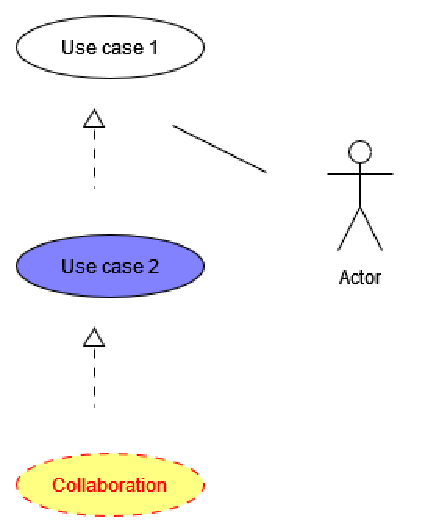
\includegraphics[scale=1.0]{test_diagram.pdf}
Aj text môže byť prezentovaný ako obrázok. Stane sa z neho označný plávajúci objekt. Po vytvorení diagramu zrušte znak \texttt{\%} pred príkazom \verb|\includegraphics| označte tento riadok ako komentár (tiež pomocou znaku \texttt{\%}).
\caption{Rozhodujúci argument.}
\label{f:rozhod}
\end{figure*}



\section{Iná časť} \label{ina}

Základným problémom je teda\ldots{} Najprv sa pozrieme na nejaké vysvetlenie (časť~\ref{ina:nejake}), a potom na ešte nejaké (časť~\ref{ina:nejake}).\footnote{Niekedy môžete potrebovať aj poznámku pod čiarou.}

Môže sa zdať, že problém vlastne nejestvuje\cite{Coplien:MPD}, ale bolo dokázané, že to tak nie je~\cite{Czarnecki:Staged, Czarnecki:Progress}. Napriek tomu, aj dnes na webe narazíme na všelijaké pochybné názory\cite{PLP-Framework}. Dôležité veci možno \emph{zdôrazniť kurzívou}.


\subsection{Nejaké vysvetlenie} \label{ina:nejake}

Niekedy treba uviesť zoznam:

\begin{itemize}
\item jedna vec
\item druhá vec
    \begin{itemize}
    \item x
    \item y
    \end{itemize}
\end{itemize}

Ten istý zoznam, len číslovaný:

\begin{enumerate}
\item jedna vec
\item druhá vec
    \begin{enumerate}
    \item x
    \item y
    \end{enumerate}
\end{enumerate}


\subsection{Ešte nejaké vysvetlenie} \label{ina:este}

\paragraph{Veľmi dôležitá poznámka.}
Niekedy je potrebné nadpisom označiť odsek. Text pokračuje hneď za nadpisom.



\section{Dôležitá časť} \label{dolezita}




\section{Ešte dôležitejšia časť} \label{dolezitejsia}




\section{Záver} \label{zaver} % prípadne iný variant názvu

\newpage

%\acknowledgement{Ak niekomu chcete poďakovať\ldots}


% týmto sa generuje zoznam literatúry z obsahu súboru literature.bib podľa toho, na čo sa v článku odkazujete
\bibliography{literature}
\bibliographystyle{plain} % prípadne alpha, abbrv alebo hociktorý iný
\end{document}
